\section{Pipeline - Remote}
\label{sec:pipeline_remote}
For the first part of the project there was a major a problem with authenticating user between the Gitea server and 
the Drone server.\\
This problem was solved by using a remote Gitea instance which could be accessed over the internet. This meant that the 
Gitea server would not be run locally on a users machine, but instead on a remote server. The Drone server, Drone runners and everything 
related to the deployment of Drone with be on the users end, hence using the users resources. This is how that deployment worked. It consisted of 
five parts:

\begin{itemize}
    \item Gitea configuration (Docker)
    \item Drone configuration (Docker)
    \item Admin (Python script)
    \item Webhook (Python script)
    \item Request script (Python script)
\end{itemize}
This solution for a pipeline had drawbacks, but that will be discussed in the section \ref{sec:discussion-pipeline}. Here
the sole focus is on how the 
product worked and how it was implemented.

\subsection{Gitea configuration}
The Gitea configuration was first created with the intention of being run locally. However, because of the Oauth2 authenticating problem, 
the Gitea server was moved to a remote server. This meant that, although it was possible to close, delete, and recreate the Gitea server with the same configuration, it was no longer necessary. 
However, this configuration made it easy to restart the server if needed.
For the deployment of the Gitea server, the following command was used:
\begin{figure}
    \begin{center}
        \centering
        \javaf{docker compose up -d}
        \caption{Docker compose command use for remote Gitea}
        \label{fig:docker-compose-remote}
    \end{center}
\end{figure}
The command showed in figure \ref{fig:docker-compose-remote} is the basic command for running Docker compose detached. 
Now behind that command is the docker-compose.yml\cite{docker-compose} file.
The docker-compose.yml file is used to define the configuration of the Gitea server. The file is shown below:
\begin{figure}[h]
    \begin{lstlisting}[style=yaml]
        version: '3'
        networks:
            kv:
                name: kv
                driver: bridge
        services:
            gitea:
                image: kraftvaerket/kv-gitea:latest
                container_name: Gitea
                restart: always
                environment:
                    - USER_UID=1000
                    - USER_GID=1000
                networks:
                    - kv
                ports:
                    - "3000:3000"
    \end{lstlisting}
\caption{docker-compose.yaml file for Gitea}
\label{sec:pipeline_remote_gitea_docker_compose}    
\end{figure}

\begin{itemize}
    \item \textbf{image}: Specifies the Docker image to use for this service, in this case, "kraftvaerket/kv-gitea:latest".
    \item \textbf{container\_name}: Specifies the name of the container, in this case, "Gitea".
    \item \textbf{restart}: Specifies the restart policy for the container, in this case, "always", which means Docker will always restart the container if it stops, regardless of the exit status.
    \item \textbf{environment}: Specifies environment variables to be passed to the container. Here, it sets the user UID and GID to 1000.
    \item \textbf{networks}: Specifies which networks this service should be connected to. In this case, it'sconnected to the "kv" network.
    \item \textbf{ports}: Specifies port mappings between the container and the host. In this case, it maps port 3000 on the host to port 3000 on the container, allowing access to the Gitea application running inside the container.
\end{itemize}
The overall of this docker-compose file is simple and basic since all of the configurations were done in the image itself.
The image used is a custom image created by the author, which 
is pulled from DockerHub. Doing all the configurations 
in the image, creates a more robust image that is more reliant to work on different machines.

This Docker compose file was then run on a \ac{Ucloud} machine which then created the Gitea server. 
To make the Gitea server accessible from the internet with another \ac{URL} than \\
\javaf{http://localhost:3000}, a reverse proxy was used called Ngrok \cite{ngrok}.
Ngrok is attached to the Gitea server by running the software running along side the Gitea server.
For that to be done you need to run the following command:
\begin{figure}[h]
    \begin{center}
        \javaf{ngrok http 3000 https://full-enormous-crow.ngrok-free.app}
    \end{center}
    \caption{Ngrok command}
    \label{fig:ngrok-command} 
\end{figure}

\begin{itemize}
    \item
    \javaf{ngrok}\\Ngrok CLI \\
    \item 
    \javaf{http 3000} \\Ngrok communicates with the Gitea server on port 3000 with the protocol http\\
    \item
    \javaf{https://full-enormous-crow.ngrok-free.app}\\Public \ac{URL} that ngrok provides
\end{itemize}

\subsection{Drone configuration}
For Drone to function, it relies on Gitea for user authentication through OAuth2. 
This means the Gitea server must be running before the Drone server can start. 
Since the Gitea server was running remotely and continuously, the Drone server could be started without any issues.

For the remote solution, it still meant that the Drone server and runners would be running locally.
The drone server is started by running a bash script, that would start the Drone server and runners.
This bash script had several functions
\begin{itemize}
    \item First:
    It checked whether all the necessary programs was installed on the machine. If not, the script would exit.
    \item Second:
    Creating a user, followed by the creation of an Oauth2 Application, for that particular user.
    The user would use these credentials to authenticate Drone with the Gitea server.
    \item Third:
    It spawned all the necessary Docker containers, both the server and the runners.
    \item Fourth:
    A newly created repository had to be activated and only after activation, it 
    was it possible to post secret and other configuration a specific repository.
    The script uses the Drone \ac{API} to activate the repository and add necessary secrets that might be used for a CTF or 
    other part of the pipeline.
    To accomplish this, the script required admin credentials for the Drone server. 
    The process involved the user logging in as an admin on the remote Gitea server, 
    authenticating as an admin on the local Drone server, and then navigating to the admin page to copy the token. 
    This token was then input into the script and used to create configurations and backend components for the Drone server.
\end{itemize}
In figure \ref{sec:pipeline_remote_drone_start_script} a snippet of the bash script is shown.
The entire script can be found in the source code under \javaf{archive/drone/drone.sh}.

\begin{figure}[h]
    \centering
    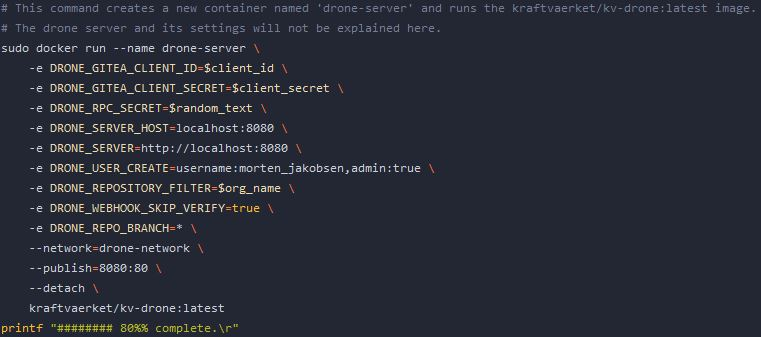
\includegraphics[scale=.69]{images/remote-script-drone.jpg}
    \caption{Drone start script snippet}
    \label{sec:pipeline_remote_drone_start_script}
\end{figure}

The image displays several environmental variables,
you see several environment variables, 
but the two most important ones are; \\ \javaf{DRONE_GITEA_CLIENT_ID} and \javaf{DRONE_GITEA_CLIENT_SECRET}. 
These variables are used to authenticate the Drone server with the Gitea server. 
While the host and RPC secrets for the Drone runners are necessary, 
the authentication credentials for OAuth2 are essential to Drone server to enable it to authenticate itself and the users 
wanting to use it.
To create the OAuth2 credentials 
on the Gitea server, a request script is utilized. This script uses the credentials provided by the user to create an OAuth2 application on the 
Gitea server for that specific user. The command in the script that executes this process is:
\begin{figure}
    \begin{center}
        \javaf{python3 ../requests/request.py $username $password}
    \end{center}
    \caption{Request script command}
    \label{fig:request-script-command}
\end{figure}
The script makes a \javaf{POST} request to the Gitea server and receives the OAuth2 credentials in return.\\
Once the pipeline was deployed and the user was created, webhooks needed to be configured. 
The purpose of the webhook is to listen for any changes in the repositories on the Gitea server. 
When a change is detected, the webhook would sends a request to the Drone server to initiate a pipeline.\\
Since the Gitea server is remote and the Drone server is local, 
an SSH tunnel is required from the remote Gitea server to the local Drone server. 
This is necessary because the Gitea server was hosted on \ac{Ucloud}, and the only way to access the machine is through SSH. 
To establish this connection, a tunnel is created from the Gitea server machine to the machine running the Drone server using the following command:\\
\begin{figure}{h}
    \begin{center}
        \javaf{ssh -Nf -L (GITEA_SERVER_MACHINES PORT):localhost:8080} \\
        \javaf{-i (SSH_KEY_FOR_LOCAL_DRONE_SERVER_MACHINE)}\\
        \javaf{USERNAME@IP_ADDRESS}
    \end{center}
    \caption{SSH tunnel command}
    \label{fig:ssh-tunnel}
\end{figure}
To establish the tunnel, the Gitea server machine needs an SSH key that can access the local machine running the Drone server. 
This is achieved by generating an SSH key on the Gitea server machine and copying the public key to the local machine.\\
Once the connection is established, a Python API on the Gitea server makes POST requests to the Drone server. 
The Gitea webhook sends a POST request to the local Flask API, which then relays the request to the Drone server.\\